%%%%%%%%%%%%%%%%%%%% author.tex %%%%%%%%%%%%%%%%%%%%%%%%%%%%%%%%%%%
%
% sample root file for your "contribution" to a proceedings volume
%
% Use this file as a template for your own input.
%
%%%%%%%%%%%%%%%% Springer %%%%%%%%%%%%%%%%%%%%%%%%%%%%%%%%%%

\documentclass{svproc}
%
% RECOMMENDED %%%%%%%%%%%%%%%%%%%%%%%%%%%%%%%%%%%%%%%%%%%%%%%%%%%
%

% to typeset URLs, URIs, and DOIs
\usepackage{url}
\usepackage{graphicx}
\usepackage{amsmath}
% \usepackage{biblatex}
\usepackage{caption}
\usepackage{subcaption}
\usepackage{tabularray}
\usepackage{array}

\newcolumntype{L}{>{\centering\arraybackslash}m{3cm}}
\def\UrlFont{\rmfamily}
\captionsetup[table]{skip=10pt}

\begin{document}
\mainmatter		 % start of a contribution
%
\title{DeepFake Detection Using Wavelet Packets with Vision Transformer
  (WPT-ViT)}
%
\titlerunning{DeepFake Detection Using WPT-ViT}
% abbreviated title (for running head)
%                                     also used for the TOC unless
%                                     \toctitle is used
%
\author{Osama Rawy \and AbdulRahman AlTahhan}
%
\authorrunning{Osama Rawy et al.} % abbreviated author list (for running head)
%
%%%% list of authors for the TOC (use if author list has to be modified)
\tocauthor{AbdulRahman AlTahhan}
%
\institute{University of Leeds, School of Computing, ODL MSc in AI, UK.\\
  WWW home page:\texttt{https://github.com/osmahus/WPT-ViT}
}

\maketitle		% typeset the title of the contribution

\begin{abstract}
  The latest advances in generative algorithms have raised the quality of
  virtually created images and videos to the point that it has become very
  difficult to distinguish the real from the generated ones (Deep-Fake). This
  stimulated hot research to build better models to detect DF.	Our paper
  proposes a new DNN model to detect DF images using a wavelet packet
  transformer
  and a vision transformer (WPT-ViT). The study shows that attention could be
  found between the WPT decompositions of an image even without slicing the
  image
  into spatial patches, which is a novel modification to the original VIT
  model.
  We showed that by using smaller model sizes and lower GPU and CPU
  requirements,
  we can achieve comparable results with previous work in this research area,
  The
  model was trained and tested using two datasets, “CIFAKE” and “140k Real and
  Fake Faces,” which are generated using StyleGAN and Stable Diffusion
  algorithms.
  % We would like to encourage you to list your keywords within
  % the abstract section using the \keywords{...} command.
  \keywords{Deep Fake Detection, Wavelet Packets, Vision Transformer}
\end{abstract}
%

\section{Introduction}
In 2014, Goodfellow et al. introduced the Generative Adversarial Network
(GAN), marking the beginning of the generative AI (GAI) era. Since then,
researchers have shifted their focus from discriminative learning to generative
learning. This wave brought various vision-generative applications to the
market, such as Midjourney, Firefly, DALL-E2, and Imagen
\cite{bengesi2024advancements}. Such applications were developed using
state-of-the-art architectures like GAN, Variational Autoencoders, and
Diffusion to generate images and videos with high fidelity and diversity,
mimicking real-world photos and videos \cite{raut2024generative}.
Vision-generative technologies have shown high value in several domains. In
the entertainment industry, for example, they could generate complete scenes
that would otherwise be very risky for actors to perform or prohibitively
expensive to produce. In Education, they could bring historical characters to
life to talk with students for an immersive learning experience; similarly, the
list of positive uses continues in other fields like manufacturing and
marketing. However, this ability to produce synthetic content with realistic
flavor was termed Deep Fake due to the unfortunate incidents in which these
technologies were used to attack people through identity theft, character
assassination, and faked pornography. On a larger scale, deep fakes were also
used to spread misinformation, fake news, and communal hatred.
According to a report released in April 2021 by Cybernews, deep fake
content over the internet doubles every six months, posing a significant threat
that needs to be addressed urgently \cite{patel2023deepfake}.
\\For that reason, there has been significant attention in both academic
and industrial fields on finding ways to detect deep fakes with high accuracy
and performance. For example, Facebook, Microsoft, and Amazon collaborated to
launch the Deep Fake Detection Challenge (DFDC) on Kaggle from 2019 to 2020. A
survey conducted by (Liang \& Xue, 2024) showed that the number of publications
on deep fake detection surpassed the number of publications on deep fake
generation in 2022 and 2023 \cite {gong2024contemporary}.
\\This paper introduces a new deepfake detection tool that combines the
strengths of wavelet analysis to extract important image features and Vision
Transformer (VIT) to create lighter models with lower GPU and CPU requirements
than CNN counterparts.

\section{Literature Review}

When it comes to detecting deep fakes, it can be seen as a binary
classification problem involving training a machine learning model on a dataset
of real and fake examples. This includes extracting relevant features from the
data and using these features to predict the authenticity of the content
\cite{patel2023deepfake}. Previous research has suggested different ways to
categorize work in the deepfake detection field. (Patel et al.,
2023)\cite{patel2023deepfake} highlighted three approaches for detecting
deepfakes in video and images.

The first approach involves using handcrafted algorithms to extract features of
visual artifacts, such as inconsistent head poses or unusual eye blinking. The
results of the feature extractor could then be passed to any classifier, such
as SVM or NN, to perform the detection. An example of this approach is the work
of Matern et al. (2019)\cite{}, which has an AUC of 0.866.

The second approach works on the pixel level to extract spatial features
related to visual inconsistencies using local feature detectors (like SIFT and
HOG) or steganography detectors. An example of this approach is the two-stream
network proposed by (Zhou et al., 2018) with an AUC of 0.927. However, the
effectiveness of the first two approaches has been reduced by the fact that the
latest deepfake datasets were created using advanced image generation
techniques, which decreases the likelihood of producing visual artifacts or
detectable local features.

The third approach utilizes Deep Neural Networks to understand the intricate
patterns and features present in the training dataset. The detection results
are more accurate when a more relevant and comprehensive dataset is provided.
According to Rana et al. (2022), previous deep fake detection models can be
grouped into three categories: Machine learning, deep learning, and
statistical. Their research indicated that 77% of the work from 2018 to 2020 falls under the Deep Learning category, with 78% being CNN-based. Ultimately, it was demonstrated that deep-learning-based deep fake detection models outperform non-deep learning models (Rana et al., 2022).

In a study conducted by Wang et al. (2024), it was demonstrated that while
Convolutional Neural Networks (CNNs) are commonly used in deepfake detection to
capture spatial relationships within images, making them effective in
identifying facial manipulations and other visual irregularities at the frame
level, Vision Transformers (ViTs) have distinct advantages in analyzing and
comprehending the intricate details of deepfake images and videos. ViTs are
especially good at understanding the overall structure of an image to identify
inconsistencies or anomalies suggestive of manipulation.

However, Wang also highlighted the challenges faced by standalone ViT models in
deepfake detection, such as their struggle to generalize across diverse
datasets, their need for extensive training data, their difficulty in
maintaining temporal consistency in video deepfakes, their limited ability to
capture local spatial information, and their potential inability to fully
capture the temporal and sequential dependencies present in video data. To
address these limitations, hybrid models that combine ViTs with other
techniques, such as CNNs or RNNs, are often utilized.

\section{Methods}
\subsection{Multiresolution Analysis}
The concept of multiresolution analysis (MRA) was developed to address the
limitations of the Fourier transform when dealing with non-stationary signals.
These limitations arise from the principle of uncertainty in the time and
frequency domains. Specifically, seeking high resolution in the time domain
leads to poor resolution in the frequency domain, and vice versa. MRA addresses
this issue by incorporating increasing levels of time samples as we transition
from the slower part of the signal to the faster part (Erick Axel, et al.).
In order to achieve this, MRA (Multiresolution Analysis) utilizes a group of
orthonormal basis functions to estimate the signals at a specific resolution.\\
% These functions are known as wavelets. The concept of orthonormal basis
% functions originated from Fourier analysis, which uses a set of sine waves to
% analyze signals. However, unlike the sine function, which oscillates
% indefinitely, the oscillation of the wavelet is confined to a finite time
% interval after which it gradually diminishes to zero. This characteristic is
% the reason behind its name "wavelet," meaning “small waves”.

% Assume that we have a discrete signal $f_m(t) \in V_m$, with a resolution $m$ 
% then we can 

% while $V_m$ is the set of all
% functions that can
% be expressed using the basis $\phi_{m,n}\left(t\right)$.\\
% And $m$ and $n$ are two integers denoting the dilation (signal resolution) and
% translation respectively, \\
% Then we can decompose $ f_m(t) $ to a lower resolution ($m-1$) by adding two
% functions $f_{m-1}(t) \in V_{m-1}$ and $e_{m-1}(t) \in W_{m-1}$
% , while $W_{m-1}$ is the orthogonal complement space of $V_{m-1}$ in ${\ V}_m$
% that includes all the functions that can be expressed using the set of
% basis $\psi_{{m-1},n}\left(t\right)$ , as follows:\\

If we have a discrete signal $f_m(t)$, with a resolution $m$
then we can decompose this signal to two functions $f_{m-1}(t)$
and $e_{m-1}(t)$ at the lower resolution $m-1$, as follows:\\

\begin{equation}
  \begin{aligned}
     & f_m(t)=\sum_{n=0}^{2^m N-1} c_{m, n} \phi_{m, n}(t)
  \end{aligned}
  \label{eq:eq1}
\end{equation}\\
then:
\begin{equation}
  \begin{aligned}
     & f_m(t)=f_{m-1}(t)+ e_{m-1}(t)
  \end{aligned}
  \label{eq:eq2}
\end{equation}\\

While:
\begin{equation}
    \begin{aligned}
       & f_{m-1}(t)=\sum_{n=0}^{2^{m-1} N-1} c_{{m-1}, n} \phi_{{m-1}, n}(t)
    \end{aligned}
    \label{eq:eq3}
  \end{equation}
  \begin{equation}
    \begin{aligned}
       & e_{m-1}(t)=\sum_{n=0}^{2^{m-1} N-1} \omega_{{m-1}, n} \psi_{{m-1}, n}(t)
    \end{aligned}
    \label{eq:eq4}
  \end{equation}\\
In general:\\ 
Let $V_m$ be the set of functions that can be expressed in terms of the basis $\phi_{m,n}$\\
,and $W_m$ be the set of functions that can be expressed in terms of the basis $\psi_{m,n}$\\

\noindent
equation \ref{eq:eq2} can be written in more general form using the orthogonal sum as follows:\\
\begin{equation}
  V_m=V_{m-1} \oplus W_{m-1}
  \label{eq:eq5}
\end{equation}\\
\noindent
by expanding equation \ref{eq:eq5} we drive the following formula:
\begin{equation}
  V_m=V_0\oplus W_0\oplus W_1\oplus ... \oplus W_{m-2}\oplus W_{m-1}
  \label{eq:eq6}
\end{equation}
\noindent
The last equation represents the m-level Discrete Wavelet Transform (DWT)
which denotes the change of basis from $\phi_m$ to the following wavelet coefficients:
\begin{equation}
  \phi_0\oplus \psi_0\oplus \psi_1\oplus ... \oplus \psi_{m-2}\oplus \psi_{m-1}
  \label{eq:eq7}
\end{equation}

\noindent
$\phi$ is wellknown as "the scaling basis" and $\psi$ is wellknown as "the wavelet basis".\\



\section{Experiment Results}
\subsection{Used Datasets}
The datasets currently used to train and test deepfake detection models,
such as FaceForensic++, Celeb-DDF, and DFDC, were developed before the latest
diffusion-based tools like DALE-2 and Midjourney came into existence. This
raises concerns about the effectiveness of models trained on traditional
datasets to detect newly created deepfake images.

Another important aspect of this study is the limitation of computational
resources, which affects the size of the required datasets. Traditional
datasets are larger than what is currently feasible. CIFAKE, which is an ideal
deepfake dataset based on CIFAR-10, addresses these concerns. Firstly, it is
created using the state-of-the-art stable-diffusion 1.3 algorithm. Secondly, it
consists of a moderate total of 120000 images, with half being real and half
being fake.

Additionally, a StyleGAN3-based dataset called "140k Real and Fake Faces" was
used to cover a broader range of deepfake styles. Similar to CIFAKE, this
dataset also has a moderate size of 140000 images, equally divided into real
and fake.

In the model code, an option was provided to split the input dataset into
training, validation, and testing according to desired split ratios. However, I
chose to keep the original split as it is for a fair comparison with other
models that are also using the same datasets.

%         \begin{figure}
%         	\centering
% 	        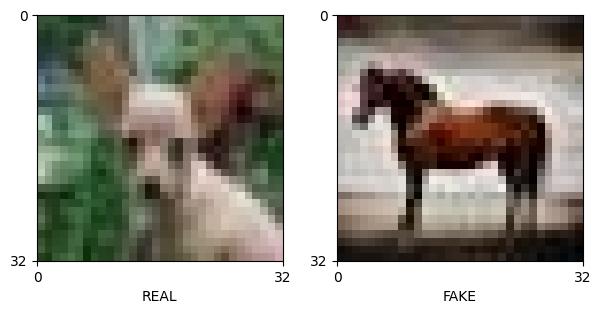
\includegraphics[scale=.5]{figures/figure_01.png}
% 	        \caption{Caption}
%           \label{fig:fig01}
%         \end{figure}
% \pagebreak

\begin{figure}
  \centering
  \begin{subfigure}{.5\textwidth}
    \centering
    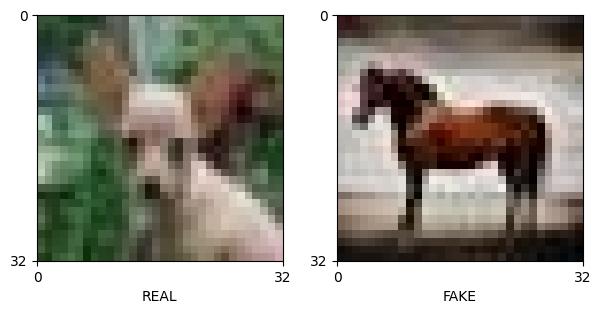
\includegraphics[width=0.9\linewidth]{figures/figure_01.png}
    \caption{CIFAKE}
    \label{fig:sub1}
  \end{subfigure}%
  \begin{subfigure}{.5\textwidth}
    \centering
    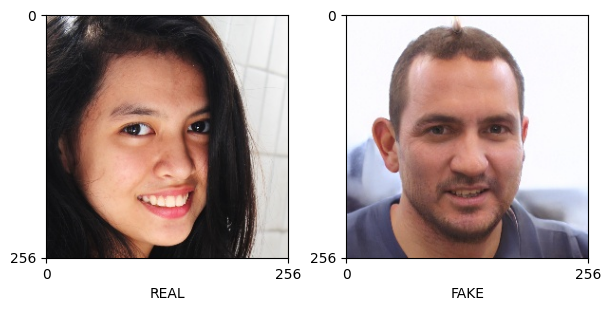
\includegraphics[width=0.9\linewidth]{figures/figure_02.png}
    \caption{140k Real and Fake Faces}
    \label{fig:sub2}
  \end{subfigure}
  \caption{The Two Used Deepfake Datasets}
  \label{fig:test}
\end{figure}
\pagebreak

\subsection{Key Packages}
The model is built using Python 3.11 , and Pytorch version 2.2.1 with cuda 12.1
The WPT stage in the WPT-ViT model is not only inspired by the work of Moritz
et al. (2024), but also uses their open wavelet library called PTWT for image
decomposition instead of the older PYWT developed by Lee et al. (2019). This
choice was made after trying both, because of the significantly faster speed of
PTWT, particularly due to its support for parallel processing using GPU (Wolter
et al., 2024).

\subsection{Experiments}
Table \ref{table:1} summarizes the trials that was made to train and evaluate
our model

\begin{table}[!ht]
  \centering
  \scalebox{0.7}{

    \begin{tabular}{|>{\centering\arraybackslash}p{0.17\linewidth}|>{\centering\arraybackslash}p{0.11\linewidth}|>{\centering\arraybackslash}p{0.11\linewidth}|>{\centering\arraybackslash}p{0.13\linewidth}|>{\centering\arraybackslash}p{0.13\linewidth}|>{\centering\arraybackslash}p{0.1\linewidth}|>{\centering\arraybackslash}p{0.11\linewidth}|>{\centering\arraybackslash}p{0.1\linewidth}|>{\centering\arraybackslash}p{0.3\linewidth}|>{\centering\arraybackslash}p{0.1\linewidth}|>{\centering\arraybackslash}p{0.1\linewidth}|}
      \hline

      \textbf{Experiment}                & \textbf{Dataset}                 &
      \textbf{Wavelet fun}               &
      \textbf{Wavelet decomp. level (L)} & \textbf{Paches per decomp. (P) } &
      \textbf{Heads (H)}                 & \textbf{Encoder levels (E) }     &
      \textbf{Sliced? (S)}               &
      \textbf{Used Slices}               & \textbf{Batch Size}              &
      \textbf{Image Dim.}
      \\
      \hline\hline

      \textbf{1}                         & CIFAKE                           &
      haar                               & 3                                & 1
                                         & 16                               & 2 & 0 & ~                     & 1000 & 32
      \\ \hline
      \textbf{2}                         & CIFAKE                           &
      db2                                & 3                                & 1
                                         & 18                               & 2 & 0 & ~                     & 1000 & 32
      \\ \hline
      \textbf{3}                         & CIFAKE                           &
      db2                                & 3                                & 1
                                         & 18                               & 2 & 0 & ~                     & 500  & 32
      \\ \hline
      \textbf{4}                         & CIFAKE                           &
      db2                                & 3                                & 1
                                         & 18                               & 1 & 0 & ~                     & 500  & 32
      \\ \hline
      \textbf{5}                         & CIFAKE                           &
      db2                                & 3                                & 1
                                         & 18                               & 1 & 0 & ~                     & 1000 & 32
      \\ \hline
      \textbf{6}                         & CIFAKE                           &
      db2                                & 3                                & 1
                                         & 18                               & 1 & 1 & [ aaa, aah, aha, haa,
      hav, hva, hvv, vaa, vav, vha ]     & 1000                             &
      32
      \\ \hline
      \textbf{7}                         & CIFAKE                           &
      db2                                & 3                                & 1
                                         & 18                               & 1 & 0 & ~                     & 2000 & 32
      \\ \hline
      \textbf{8}                         & RVSF                             &
      haar                               & 3                                & 1
                                         & 16                               & 2 & 0 & ~                     & 1000 & 32
      \\ \hline

    \end{tabular}}

  \caption{Table Shows}
  \label{table:1}
\end{table}

\subsubsection{Experiment 1}



%
% ---- Bibliography ----
%
\begin{thebibliography}{6}
  %

  \bibitem{bengesi2024advancements}
  Bengesi, Staphord, et al. "Advancements in Generative AI: A Comprehensive
  Review of GANs, GPT, Autoencoders, Diffusion Model, and Transformers." IEEE
  Access (2024).

  \bibitem{raut2024generative}
  Raut, Gaurav, and Apoorv Singh. "Generative AI in Vision: A Survey on Models,
  Metrics, and Applications." arXiv preprint arXiv:2402.16369 (2024).

  \bibitem{patel2023deepfake}
  Pei, Gan, Jiangning, Zhang, Menghan, Hu, Guangtao, Zhai, Chengjie, Wang,
  Zhenyu, Zhang, Jian, Yang, Chunhua, Shen, Dacheng, Tao. "Deepfake Generation
  and Detection: A Benchmark and Survey". arXiv preprint arXiv:2403.17881.
  (2024).

  \bibitem {gong2024contemporary}
  Gong, Liang Yu, Xue Jun, Li. "A Contemporary Survey on Deepfake Detection:
  Datasets, Algorithms, and Challenges". Electronics 13. 3(2024): 585.

  \bibitem{zhang2022deepfake}
  Heidari, Arash, Nima, Jafari Navimipour, Hasan, Dag, Mehmet, Unal. "Deepfake
  detection using deep learning methods: A systematic and comprehensive
  review".
  Wiley Interdisciplinary Reviews: Data Mining and Knowledge Discovery 14.
  2(2024): e1520.

  \bibitem{rana2022deepfake}
  Patel, Yogesh, Sudeep, Tanwar, Rajesh, Gupta, Pronaya, Bhattacharya, Innocent
  Ewean, Davidson, Royi, Nyameko, Srinivas, Aluvala, Vrince, Vimal. "Deepfake
  Generation and Detection: Case Study and Challenges". IEEE Access. (2023).

  %   \bibitem{akhtar2023deepfakes}
  %   Zhang, Tao. "Deepfake generation and detection, a survey". Multimedia Tools and Applications 81. 5(2022): 6259–6276.

  %   \bibitem{masood2023deepfakes}
  %   Akhtar, Zahid. "Deepfakes generation and detection: A short survey". Journal of Imaging 9. 1(2023): 18.

  %   \bibitem{stroebel2023systematic}
  %   Rana, Md Shohel, Mohammad Nur, Nobi, Beddhu, Murali, Andrew H, Sung. "Deepfake detection: A systematic literature review". IEEE access 10. (2022): 25494–25513.

  %   \bibitem {heidari2024deepfake}
  %   Masood, Momina, Mariam, Nawaz, Khalid Mahmood, Malik, Ali, Javed, Aun, Irtaza, Hafiz, Malik. "Deepfakes generation and detection: State-of-the-art, open challenges, countermeasures, and way forward". Applied intelligence 53. 4(2023): 3974–4026.

  %   \bibitem {pei2024deepfake}
  %   Stroebel, Laura, Mark, Llewellyn, Tricia, Hartley, Tsui Shan, Ip, Mohiuddin, Ahmed. "A systematic literature review on the effectiveness of deepfake detection techniques". Journal of Cyber Security Technology 7. 2(2023): 83–113.

  %   \bibitem {wang2024timely}
  %   Wang, Zhikan, Zhongyao, Cheng, Jiajie, Xiong, Xun, Xu, Tianrui, Li, Bharadwaj, Veeravalli, Xulei, Yang. "A Timely Survey on Vision Transformer for Deepfake Detection". arXiv preprint arXiv:2405.08463. (2024).

  % \bibitem {140krvsf}	
  % “140k Real and Fake Faces | Kaggle.\url{https://www.kaggle.com/xhlulu/140k-real-and-fake-faces}

\end{thebibliography}
\end{document}
